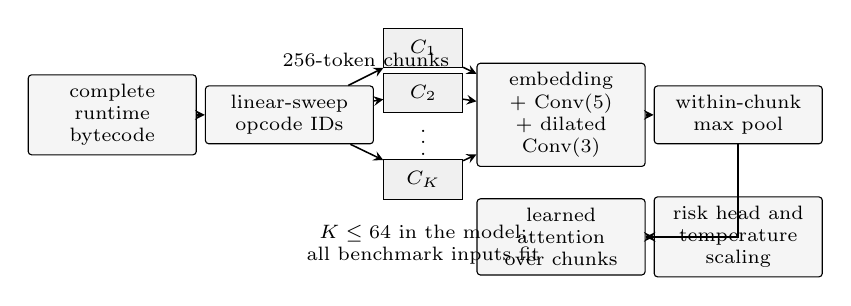
\begin{tikzpicture}[
  font=\scriptsize,
  box/.style={draw, rounded corners=1.2pt, minimum height=7mm, text width=19mm,
              align=center, fill=gray!8},
  small/.style={draw, minimum height=5mm, minimum width=10mm, align=center, fill=gray!12},
  flow/.style={->, >=stealth, line width=.55pt}
]
  \node[box] (bytecode) at (-3.6,0) {complete runtime bytecode};
  \node[box] (tokens) at (-1.35,0) {linear-sweep opcode IDs};
  \node[small] (c1) at (.35,.85) {$C_1$};
  \node[small] (c2) at (.35,.28) {$C_2$};
  \node at (.35,-.25) {$\vdots$};
  \node[small] (ck) at (.35,-.82) {$C_K$};
  \node[box] (local) at (2.10,0) {embedding $+$ Conv(5) $+$ dilated Conv(3)};
  \node[box] (pool) at (4.35,0) {within-chunk max pool};
  \node[box] (attn) at (2.10,-1.55) {learned attention over chunks};
  \node[box] (head) at (4.35,-1.55) {risk head and temperature scaling};
  \draw[flow] (bytecode) -- (tokens);
  \draw[flow] (tokens) -- node[above]{256-token chunks} (c1);
  \draw[flow] (tokens) -- (c2);
  \draw[flow] (tokens) -- (ck);
  \draw[flow] (c1) -- (local);
  \draw[flow] (c2) -- (local);
  \draw[flow] (ck) -- (local);
  \draw[flow] (local) -- (pool);
  \draw[flow] (pool.south) |- (attn.east);
  \draw[flow] (attn) -- (head);
  \node[align=center] at (.35,-1.65) {$K\leq64$ in the model;\\all benchmark inputs fit};
\end{tikzpicture}

